When designing the analog circuitry the topology as well as the technological limitations for production was taken from~\cite{oppgave}.
This section therefore focuses on the physical dimensions of the different components as specified in figures~\ref{fig:implpixel}~and~\ref{fig:implcamera}.

The most important property of the analog pixel is that the charge stored over CS remains unchanged while being read,
the transistors M1 and M2 must therefore be tuned for minimal leakage current as described in Section~\ref{sec:leakagecurrent}.
The transistor M4 must be tuned in the same way to avoid any interference between P11 and P21 as well as between P12 and P22 during readout as shown in figure~\ref{fig:implcamera}.

The current source transistors MC1 and MC2 must be tuned for the quickest possible response of the current source, this is in order to get the fastest possible stable output when reading from a pixel.
They are therefore tuned for maximum current throughput as explained in Section~\ref{sec:leakagecurrent} and verified in Section~\ref{sec:Simulations}.

The capacitor CS and transistor M3 are tuned to empirically found values as shown in Section~\ref{sec:Simulations} in order to give the best dynamic range of the pixel
as a function of lighting conditions and exposure time.

All component values are shown in table~\ref{tab:componentvalues}.

\begin{table}[htbp]
  \centering
  \caption{Physical values of components}
  \subcaption*{Panel A: transistors}
  \begin{tabular}{ c | c c }
    Component & W & L \\
    \midrule
    M1 & $1.08\mu$ & $1.08\mu$ \\
    M2 & $1.08\mu$ & $1.08\mu$ \\
    M3 & $3.00\mu$ & $0.67\mu$ \\
    M4 & $1.08\mu$ & $1.08\mu$ \\
    MC1 & $5.04\mu$ & $0.36\mu$ \\
    MC2 & $5.04\mu$ & $0.36\mu$
  \end{tabular}
  \bigskip
  \subcaption*{Panel B: capacitors}
  \begin{tabular}{c | c}
    Component & C \\
    \midrule
    CS & $2.5pF$ \\
    CC1 & $3.0pF$ \\
    CC2 & $3.0pF$
  \end{tabular} \label{tab:componentvalues}
\end{table}


\begin{figure}[htbp]
  \centering
  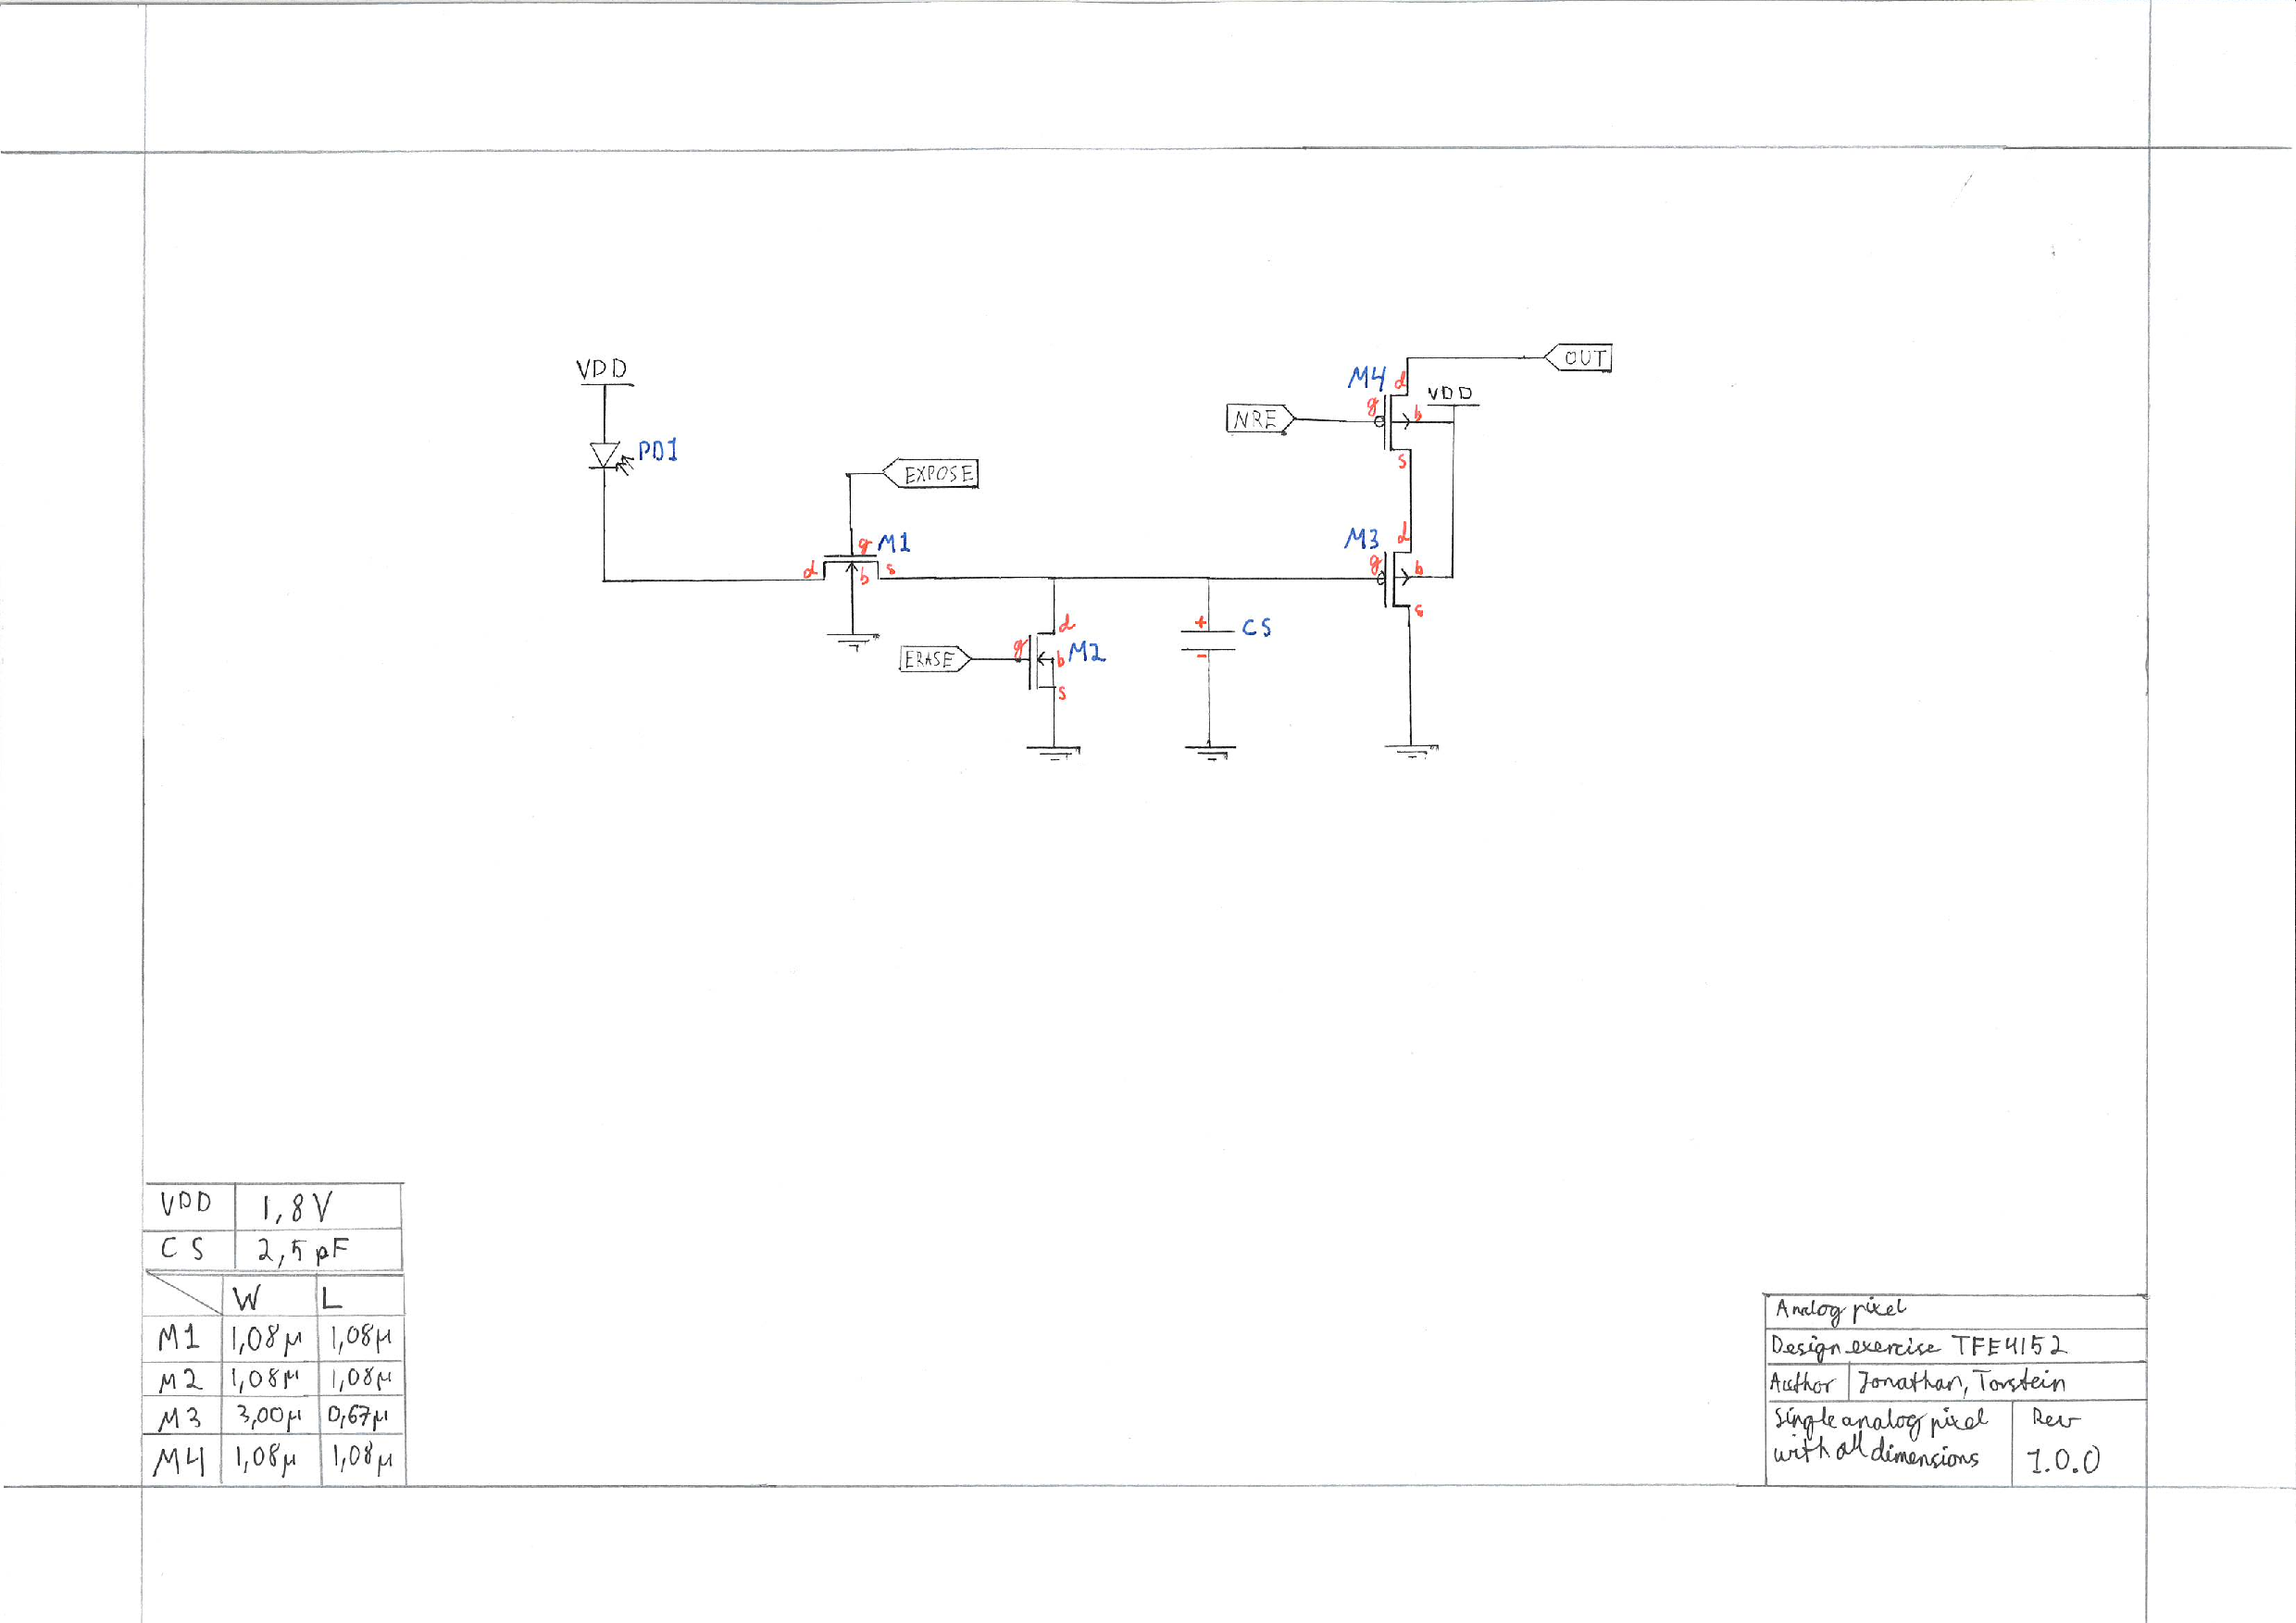
\includegraphics[width=0.85\textwidth]{figures/SchematicPixel}
  \caption{Implementation of one pixel, figure allso exist in Appendix~\ref{ap:Schematics}}
  \label{fig:implpixel}
\end{figure}
\begin{figure}[htbp]
  \centering
  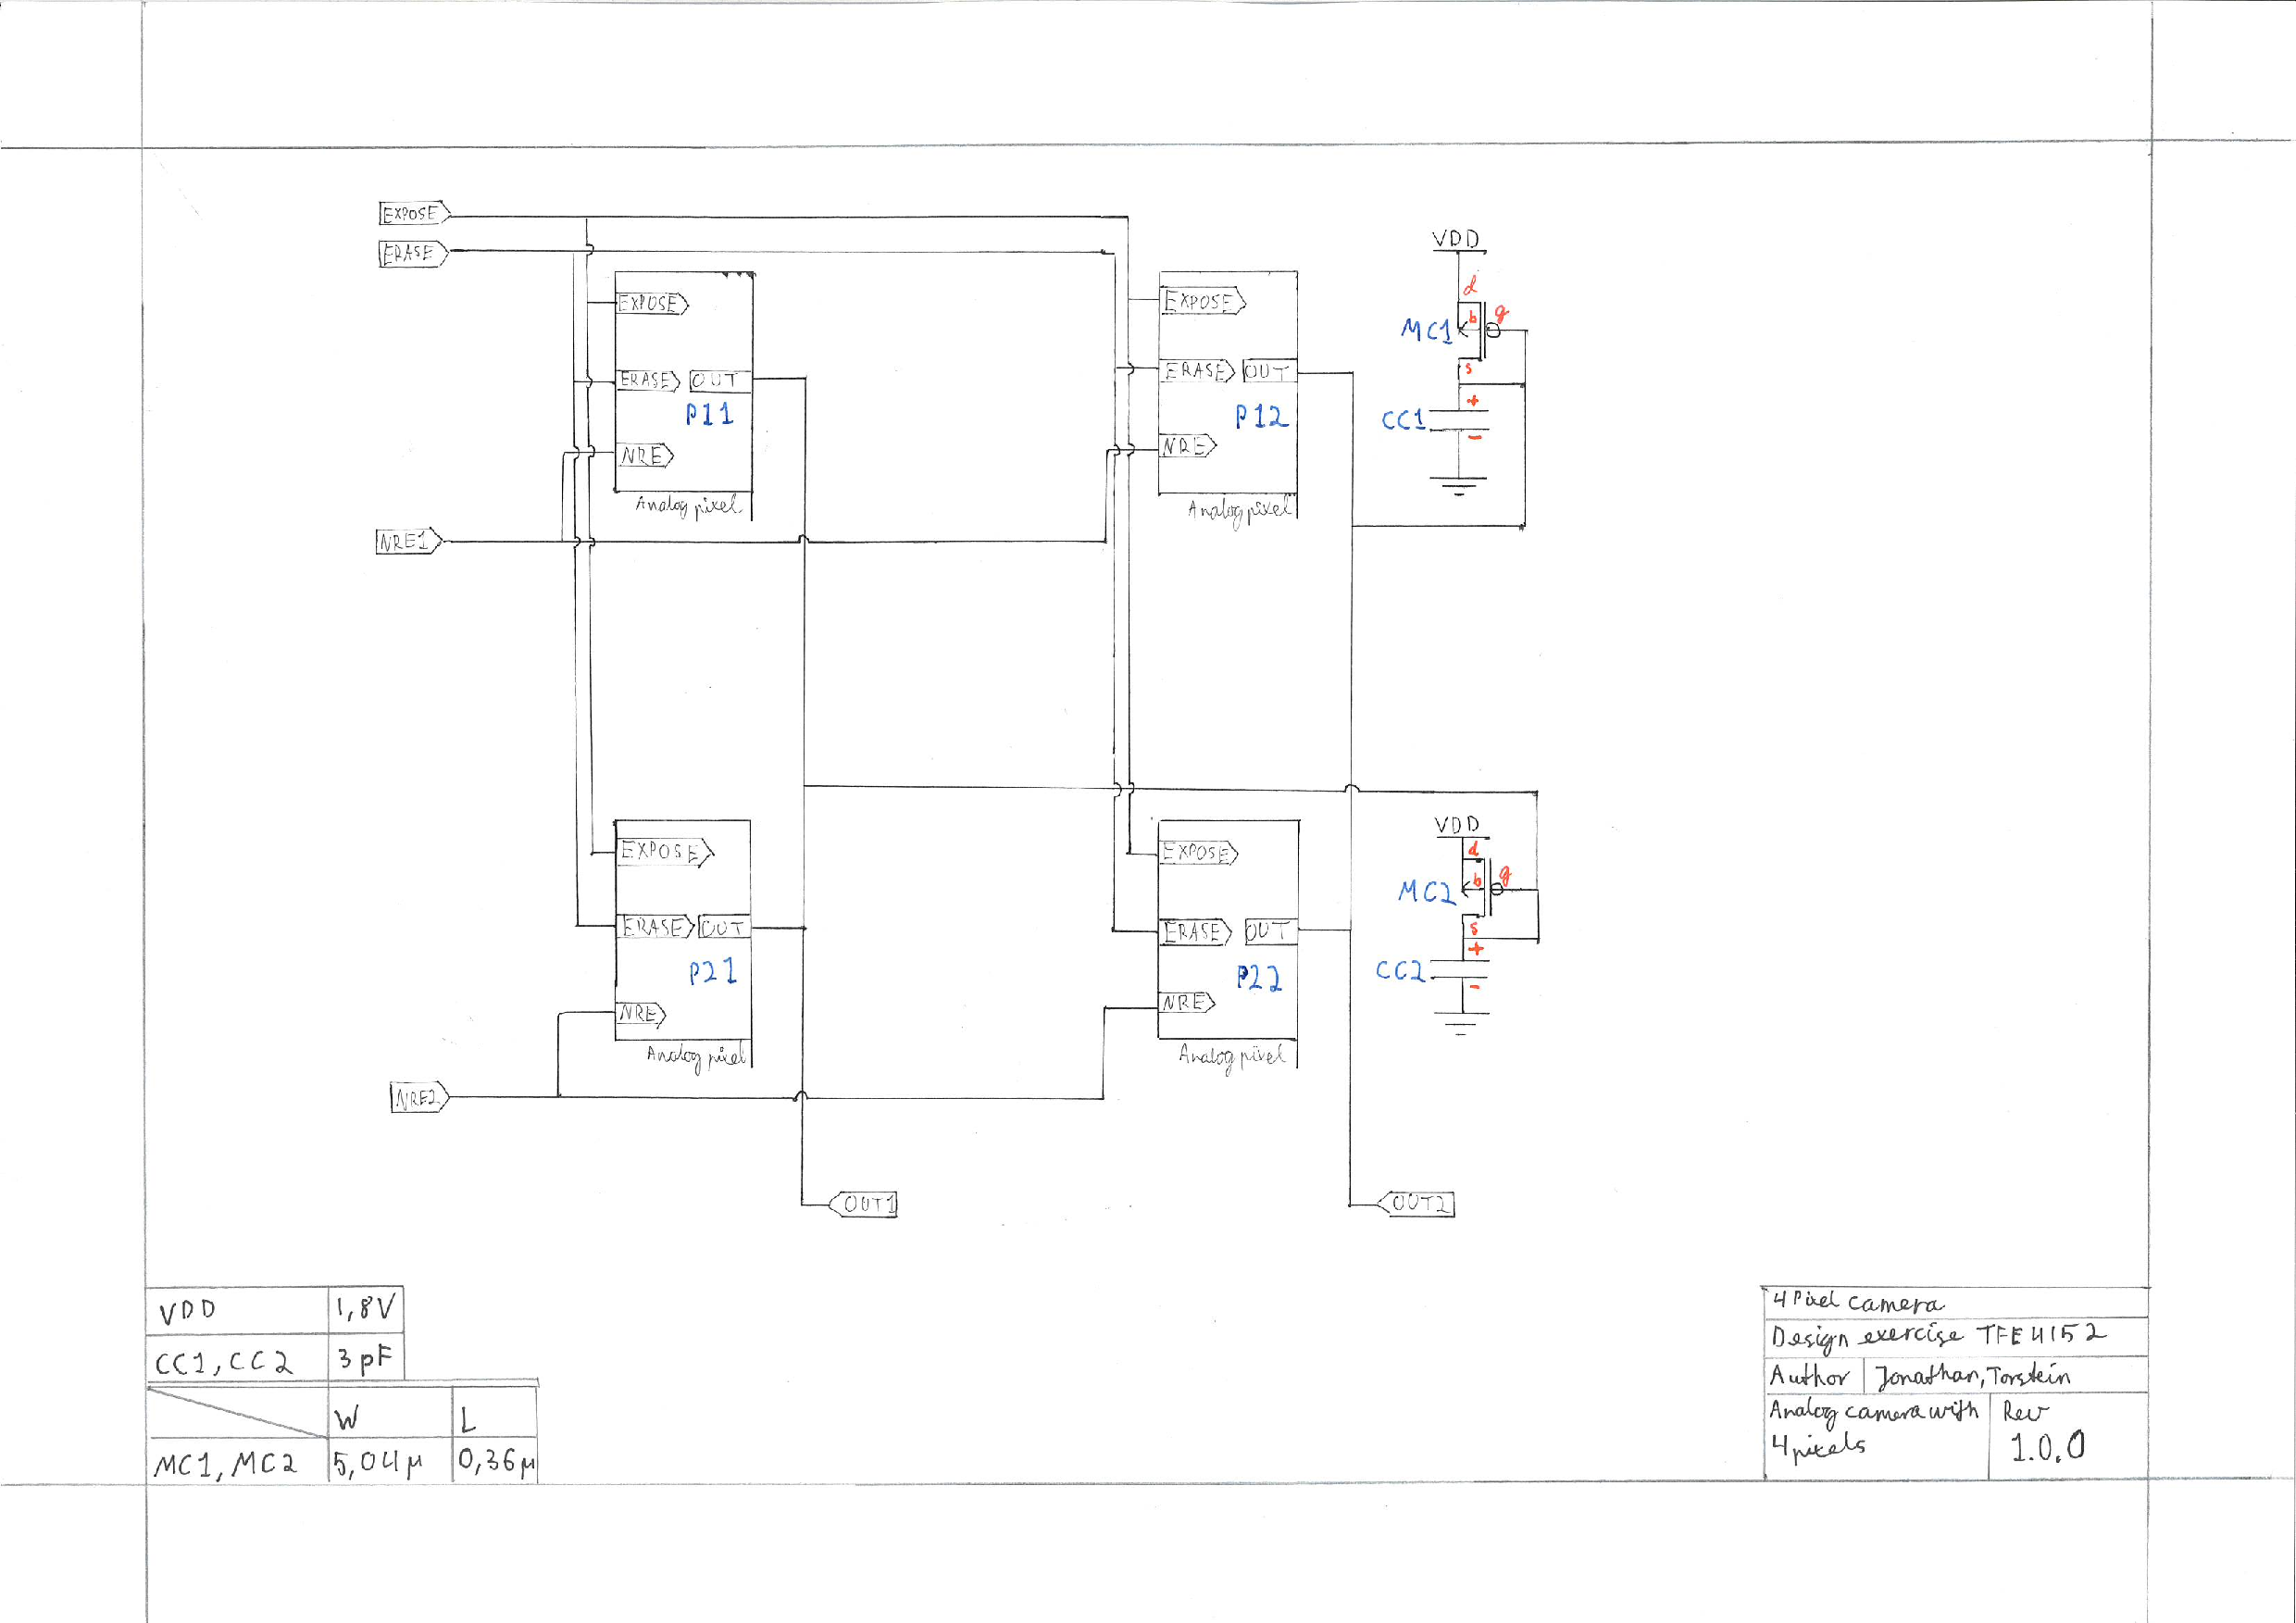
\includegraphics[width=0.85\textwidth]{figures/SchematicCamera}
  \caption{Implementation of the analog part of the camera, figure allso exist in Appendix~\ref{ap:Schematics}}
  \label{fig:implcamera}
\end{figure}